\documentclass[journal]{IEEEtran}
\usepackage{fullpage,enumitem,amsfonts,amsmath,amssymb,graphicx,cite,hyperref}

\begin{document}
\title{Personal Legal Counselor and Interpreter of the Law via Machine Learning}
\author{Derek Yan, Tianyi Wang, Patrick Chase\\
\{zhyan, tianyiw, pchase\}@stanford.edu}
\markboth{Final report for CS229, Fall 2014}
{Shell \MakeLowercase{\textit{et al.}}: Personal Legal Counselor and Interpreter of the Law via Machine Learning}
\maketitle

\begin{abstract}
The goal of this project was to predict the likelihood of winning a new legal dispute based on results of past cases. We collected over 5000 legal proceedings in the form of case briefs from the internet and used various language processing techniques to parse the raw text into feature vectors. We then used this feature vectors to train several binary classification algorithms, including Naive Bayes, random forrests, logistic regression and an SVM. The SVM model achieved the highest test set accuracy of 62\%, which was an improvement over the random 50\% baseline. In this paper, we explain the details of how we transformed the raw text of the case briefs into feature vectors, and how we used them to build several models for prediction. We then discuss the results obtained by each of the models and suggest future work that could be done in the area.
\end{abstract}

\begin{keywords}
law, machine learning, case briefs, court cases.
\end{keywords}

\section{Introduction}
\IEEEPARstart{``T} he first thing we do, let's kill all the lawyers'' - William Shakespeare, 2 Henry VI, 4.2.59. 

Any major transaction, legal procedure, or patent dispute always requires an attorney-at-law in the due process. However, paying an attorney, even for a consultation, can be too expensive and out of reach for much of the population. Due to the exorbitant cost of legal action, many cases are unresolved or dropped. Our goal was to create a tool that would provide legal counsel to people who would otherwise not have access to it. In particular, our model would tell someone the probability they have of winning a given case, which would allow them to make the a better decision of whether or not to pursue further legal action. 

\section{Dataset}

Our dataset was obtained from \url{www.casebriefs.com}. It consisted of 5,836 legal case briefs, where each case brief was split up into four segments of text, the \textit{Parties in Dispute}, the \textit{Summary of Facts}, the \textit{Issue of Law}, and the \textit{Verdict}. Fig. \ref{ExampleCaseBrief} is  an example of a very short case brief.

\begin{figure}
    \centering
    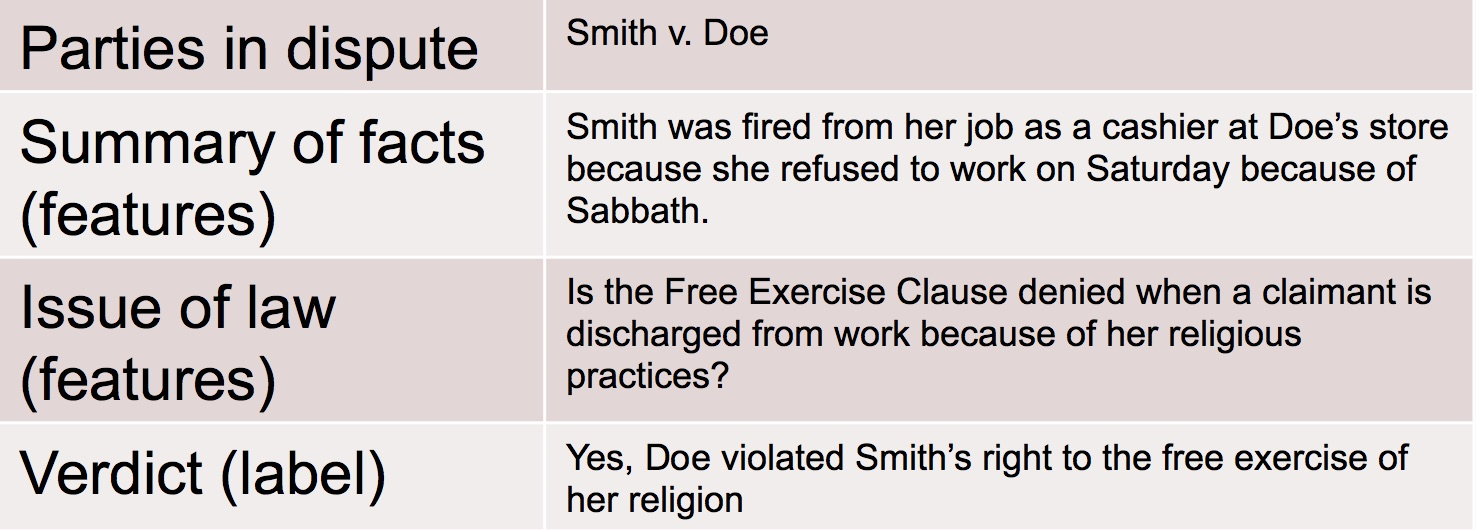
\includegraphics[width=3.5in]{exampleCaseBrief.jpg}
    \caption{Example Case Brief}
    \label{ExampleCaseBrief}
\end{figure}

\section{Baseline and Oracle Results}
Before tackling the actual problem. We first considered taking the baseline and oracle results of the legal case predictor. The baseline solution was using linear regression to serve as a predictor of future cases. We used 3-grams from the input text for feature extraction.  When the new input was given, we extracted the features, and then used stochastic gradient descent to come up the learn-predictor to estimate the likelihood of the plaintiff winning the case. For the test data, we had an error rate of around 49\%. Using word features only got us around 51\% of correct prediction.

The oracle was a manual interpretation of facts and issues given a test case by the group members. We read over the facts of a legal proceeding, the interpretation of law which was under question, and used our common sense to give a probable decision. For legal matters that were not familiar to us, we would research laws of such matter and make human predictions. This would serve as our oracle. The test error would be small but still non- negligible because the group members are not of the legal profession. For our test cases of 20, we had an error rate of 10\%. 

\section{Features and Preprocessing}

First, we parsed the \textit{Verdict} section to obtain the binary labels for the cases. When the \textit{Verdict} was held, meaning the answer to the \textit{Issue of Law} was "yes," we gave a positive label to the example, but when the answer to the \textit{Issue of Law} was "no" we gave a negative label to the example. 

After extracting the labels, we found that there were 2099 positive cases and 3737 negative cases.

\subsection{Training and Testing Data}

We then split up the data into the training and testing datasets described below.

\begin{table}[ht]
\centering
\begin{tabular}{rrr}
  \hline
& Training Dataset &	Testing Dataset\\
  \hline
Total Examples&	3800&	400 \\
Positive Examples &	1900 &	200 \\
Negative Examples &	1900 &	200 \\
   \hline
\end{tabular}
\end{table}

\subsection{Feature Generation}

To create the feature vectors, we used the \textit{Summary of Facts} section and \textit{Issue of Law} section. We did not use any of the text from the \textit{Verdict} section because that section was used to determine the positive or negative label.

First, we processed the raw text of the case briefs by transforming each word to its stem using the Lancaster Stemmer from the NLTK, Natural Language ToolKit \cite{Loper:2002:NNL:1118108.1118117}. We then formed a dictionary by scanning through all the words in our dataset. After forming the dictionary, we used the dictionary to represent the case briefs using the bag-of-words representation. In our representation, the $i$th element of the feature vector for an example corresponded to the number of times the $i$th stem occurred in the given case brief.

We also experimented with adding bigrams and trigrams to the feature vectors. For the algorithms that took dense matrices as input, this made the input too large and cause the algorithms to take too long or run out of memory. However, the SVM implementation took in a sparse matrix input and this was able to run with bigrams and trigrams.

(Add part of example feature vector?)

\section{Models}

For all the models we used the SciKit-Learn package \cite{scikit-learn} for python.

\subsection{Naive Bayes}

The implementation of Naive Bayes that we used assumed that the likelihood of the features was normally distributed:

\begin{equation}
\begin{aligned}
p(x_i | y) = \frac{1}{\sqrt{2 \pi \sigma_y^2}} \exp \left ( - \frac{(x_i - \mu_y)^2}{2\sigma_y^2}\right)
\end{aligned}
\end{equation}

There were no other parameters to set for Naive Bayes, so after choosing the distribution to represent the likelihood of the features, we trained our model.

\subsection{Random Forests}

When we first ran the out of the box random forest classifier from SciKit-Learn, we got an accuracy on the training set of 97\% and an accuracy on the testing set of around 53\%, illustrating that we were overfitting the training data. To remedy this issue, we set the max depth of the tree to be 7, which greatly improved our model. 

\subsection{Logistic Regression}

When modeling the outcome of a legal case with logistic regression, we had the same issue with the out of the box algorithm. We were drastically overfitting the training data, which led to a poor accuracy on the training set. To fix this issue we used a logistic regression model with L2 regularization. This decreased our training set accuracy from 99\% to 67\%, and improved the performance of the model on the testing dataset. 

\subsection{SVM}

Details on SVM.

\section{Results}

Large table of results and confusion matrices.

Important words/phrases

\section{Discussion}

Legal proceeding labels are subjective in the sense that ruling are influenced by the sentiment of the jury and may not be captured fully in case briefs [2]. An oracle of manually studying a dispute and researching online to give a well-informed prediction only results in a correctness of 90\%. Feature set can be improved by collaborating with legal professionals to add nuances and hand-select features
Future work can be done on factor graph to improve correctness. Aspects such as demographics of the jury, state of the trial, time of the proceedings can be used.



\section{Conclusions}

Legal dispute outcome was predicted with an accuracy of around 62\% based on past court findings using machine learning techniques. Past proceedings in the form of case briefs were used to extract features and labels. Feature extractor used techniques in NLP to remove word stems and map words of similar categories. The features that we used in the end were word grams with length 1, 2 and 3. The labels were the verdicts of the proceeding. Naive Bayes, Random Forests, Logistic Regression and SVM were the four models used for prediction. Ten fold cross validation was used for training and testing. Each model had similar accuracy around 62\% while training error was also around 64\%. 




\section{Related Work}

Machine Learning in law is relatively an untapped market. There currently is not a predictor based on past legal proceedings. With that being said, there are two existing websites that offer services in law through machine learning:

\textit{FindLaw.com}: A website that allows users to search for relevant lawyers based on legal needs and  provide legal counseling through a forum. A recommendation system is used for picking which lawyer is more relevant for the case at hand.

\textit{Judicata}: Mapping unstructured legal data into a generative model to empower lawyers to find the most relevant and convincing past proceedings. This information then can be used to support an argument in court.

\section{Future Work}

\begin{thebibliography}{1}

\bibitem{IEEEhowto:kopka}
H.~Kopka and P.~W. Daly, \emph{A Guide to \LaTeX}, 3rd~ed.\hskip 1em plus
  0.5em minus 0.4em\relax Harlow, England: Addison-Wesley, 1999.
  \bibitem{IEEEhowto:kopka}
  B. M. McKimmie et al, “Objective and Subjective Comprehensions of Jury Instructions in Criminal Trials” in \textit{New Criminal Law Review}, Vol. 17., Number 2. University of California: pps 163-183. 


\end{thebibliography}


\end{document}

